\documentclass{article}
\usepackage[utf8]{inputenc}
\usepackage{graphicx}
\usepackage{fancyvrb}
\usepackage[T1]{fontenc}
\usepackage{lmodern}
\usepackage{hyperref}
\usepackage{xcolor}
\usepackage{verbatim}
\usepackage{amsthm}
\usepackage{amsmath}
\usepackage{caption}
\usepackage{textcomp}
\usepackage{float}

\newcommand{\resource}[1]{(Local copy saved to \texttt{#1})}
\newcommand{\tttilde}[0]{\textasciitilde{}}
\newcommand{\todo}[1]{{\color{blue}{TODO: #1}}}

\theoremstyle{definition}
\newtheorem{program}{Program}
\newtheorem{exercise}{Exercise}

\begin{document}

\section{Background}
This document introduces OpenMP (Open Multi-Processing), a framework for writing multithreaded parallel C programs. OpenMP has an emphasis on encouraging efficient memory sharing between threads on the same machine. Thus, the degree of parallelism available to an OpenMP program is generally limited to the number of cores on one machine. 

The following assumes familiarity with using a terminal, as well as the ability to connect to the SECS Linux servers from a terminal using SSH.

\textbf{Note:} The SECS server \texttt{ringo.secs.oakland.edu} should be used for this assignment, which relies on a version of OpenMP that is only implemented in more recent versions of the \texttt{gcc} compiler. SECS servers other than Ringo may not have an up-to-date version of \texttt{gcc} installed.

\section{Hello World in OpenMP}

This section will present the simple "Hello World" program \texttt{omp-hello-world.c}, which uses the OpenMP interface. This program demonstrates two functions which are a fundamental part of the OpenMP API:
\begin{itemize}
    \item \texttt{omp\_get\_thread\_num()} returns the calling thread's unique thread ID. 
    
    \item \texttt{omp\_get\_num\_threads()} returns the total number of allocated threads at the time the function is called.
\end{itemize}

This program also demonstrates the use of OpenMP \emph{compiler directives}, which usually represent most of the functionality in an OpenMP program. Compiler directives are used to parallelize \emph{structured blocks} in an OpenMP program, where a structured block is any block of code with exactly one entry point and one exit point. An OpenMP compiler directive has the syntax:
\begin{verbatim}
#pragma omp [construct] [clauses]
\end{verbatim}
The value of \texttt{construct} describes the behavior of the directive. Different constructs are analagous to the different functions in a traditional API. Likewise, the directive's \texttt{clauses} modify the behavior of the construct, analagous to a function's arguments.

The compiler directive used in the example program invokes the \texttt{parallel} construct with the following statement:
\begin{verbatim}
#pragma omp parallel private(tid)
\end{verbatim}

The \texttt{parallel} construct creates a number of threads, all of which immediately begin executing the structured block under the directive in parallel. There are several ways to set the number of threads created, but the two most common ways are the following:

\begin{enumerate}
    \item The \texttt{num\_threads} clause controls the number of created threads if present. For example, the following directive would always create 4 threads:\\
    \texttt{\#pragma omp parallel num\_threads(4)}
    
    \item If no \texttt{num\_threads} clause is present, the terminal environment variable \texttt{OMP\_NUM\_THREADS} controls the number of created threads.
\end{enumerate}

Since the example program doesn't have a \texttt{num\_threads} clause, the \texttt{OMP\_NUM\_THREADS} environment variable can be used to set the number of threads.

The compiler directive in \texttt{omp-hello-world.c} also uses the \texttt{private(tid)} clause, which allocates private copies of the variable \texttt{tid} for each thread created by the directive. Without creating private copies of \texttt{tid}, the program would have a race condition, since the shared value of \texttt{tid} could be overwritten before a thread has time to print its own value. In practice, this program is small enough that this race condition is unlikely to occur, so the use of the \texttt{private} clause is mainly to demonstrate best practices: whenever each thread needs its own copy of a variable, that variable should be marked private.

\begin{exercise}
Compile the \texttt{omp-hello-world.c} program using the \texttt{gcc} compiler, then execute the result. The \texttt{-fopenmp} argument needs to be passed to \texttt{gcc} to compile an OpenMP program:

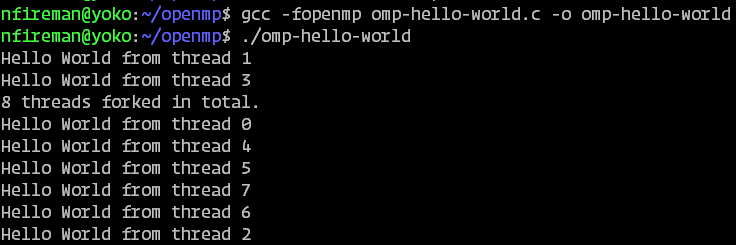
\includegraphics[width=\textwidth]{images/hello-world-output.png}

Note that the number of threads created isn't being explicitly set, and will vary depending on the environment default value.
\end{exercise}

\begin{exercise}
Explicitly set the environment variable \texttt{OMP\_NUM\_THREADS} to 4 using the \texttt{export} terminal command, then execute \texttt{omp-hello-world} again.

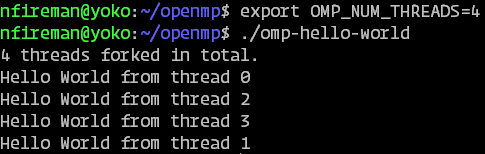
\includegraphics[width=\textwidth]{images/hello-world-export-output.png}
\end{exercise}

\subsection*{Additional resources}

\begin{itemize}
    \item Slides from an introductory OpenMP presentation:
    
    \url{https://www.openmp.org/wp-content/uploads/omp-hands-on-SC08.pdf}
    
    \resource{resources/omp-hands-on-SC08.pdf}
    
    \item An online OpenMP tutorial published by the Lawrence Livermore National Laboratory:
    
    \url{https://hpc.llnl.gov/openmp-tutorial}
    
    \resource{resources/OpenMP\_Tutorial.pdf}
\end{itemize}

\section{Selection sort}

\begin{figure}
    \centering
    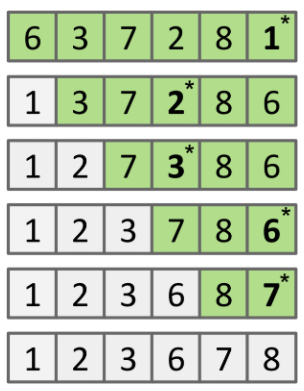
\includegraphics{images/selection-sort.png}
    \caption{Selection sort. A bold number indicates the minimum unsorted value.\\
    \textbf{Source}: https://courses.cs.washington.edu/courses/cse373/19au/lectures/05/reading/}
    \label{fig/selection-sort}
\end{figure}

This section presents a selection sort algorithm that has been parallelized using OpenMP. The selection sort algorithm is demonstrated in Figure \ref{fig/selection-sort}. At the beginning of the algorithm the entire array is assumed to be unsorted, and selection sort proceeds to sort the array one element at a time from left to right. At each step, the unsorted section is searched to find its minimum element, and that minimum is swapped to the beginning of the unsorted section, where it will be correctly sorted. This process continues until the entire array is sorted.

The algorithm can be understood as two nested for loops, where the outer loop iterates over the elements of the array, and the inner loop finds the minimum element of the unsorted section. Assuming the input array is named \texttt{data} and has length \texttt{N}, we have the following code:

\begin{figure}[H]
\begin{verbatim}
for (int i = 0; i < N; i++) {
    // initialize the minimum to the first unsorted element
    int min_index = i;
    int min_value = data[i];
    
    // search the remaining unsorted portion for its minimum
    for (int j = i + 1; j < N; j++) {
        if (data[j] < min_value) {
            min_index = j;
            min_value = data[j];
        }
    }
    
    // swap the minimum value to the front of the unsorted section
    swap(&data[i], &data[min_index]);
}
\end{verbatim}
\end{figure}

When trying to parallelize this algorithm, we first note that the outer \texttt{for} loop cannot be parallelized. This is because the array is changed at the end of each outer loop iteration (via the swap), meaning that a given outer loop iteration cannot begin until the previous iteration has ended.

The inner \texttt{for} loop, however, only searches a subarray for its minimum element, which is an operation that can be parallelized. We will assign multiple threads to search part of the subarray for that part's minimum value. Then, the minimum value of the entire subarray can be computed as the smallest among the minima found by each thread. This can be implemented as a \emph{reduction}, an OpenMP clause used to combine one value computed by each thread into a single value.

As a brief summary of reductions, the following program computes the sum of the values in the array \texttt{data}, storing it in the variable \texttt{sum}:
\begin{verbatim}
int sum = 0;
#pragma omp parallel for reduction(+:sum)
for (int i = 0; i < N; i++) {
    sum += data[i]
}
\end{verbatim}

The clause \texttt{reduction(+:sum)} tells OpenMP to compute the sum (indicated by \texttt{+}) of each thread's partial result stored in the \texttt{sum} variable. Notice that if the compiler directive were removed, the remaining program would still compute the sum serially. This demonstrates a very useful feature of the design of OpenMP: often, a serial program can be parallelized solely through compiler directives, without the programmer needing to modify the original program's logic.

Returning to selection sort, we could make use of the built-in \texttt{min} reduction operation, which could be used to compute the minimum unsorted value as desired:

\begin{figure}[H]
\begin{verbatim}
#pragma omp parallel for reduction(min:min_value)
for (int j = i + 1; j < n; j++) {
  if (data[j] < min_value) {
    min_value = data[j];
  }
}
\end{verbatim}
\end{figure}

The issue with this approach is that we no longer record the index where \texttt{min\_value} was found. Recall that the index of the minimum value is necessary, since after locating the minimum, we then need to swap it to the beginning of the unsorted section of the array.

One solution to this problem is to implement a \emph{user-defined reduction} operation which computes the minimum value while also recording the index where that value was found. First, we define a \texttt{struct} that encodes both a value and its index in the array:
\begin{verbatim}
typedef struct entry {
  int index;
  int value;
} entry;
\end{verbatim}

Next, we declare a reduction operation that computes the minimum of two \texttt{entry} instances by comparing their \texttt{value} fields:

\begin{verbatim}
#pragma omp declare reduction(min_entry : entry : \
  omp_out = (omp_in.value < omp_out.value) ? omp_in : omp_out)
\end{verbatim}

The above \texttt{declare reduction} directive has three colon-separated arguments, described as follows. Note that the \texttt{\textbackslash} character on the first line escapes the line break, allowing the declaration to span two lines for clarity.

\begin{itemize}
    \item The first argument \texttt{min\_entry} is the name of the declared reduction operation. 
    
    \item The second argument \texttt{entry} is the data type of the values being combined (the \texttt{struct} defined above).
    
    \item The third argument is an expression that describes how OpenMP should combine two values of the type \texttt{entry}. By convention, the two values have the names \texttt{omp\_in} and \texttt{omp\_out}, and the combined value must be written to \texttt{omp\_out}. 
\end{itemize}

The expression given in the third argument compares the \texttt{value} fields of the two structs, and writes the struct with the smaller \texttt{value} field to \texttt{omp\_out}. When a sequence of \texttt{entry} values are combined in this way, the final result will thus contain the minimum out of all \texttt{value} fields.

With this reduction operation defined, we can simply add a corresponding compiler directive to the inner loop discussed above, and OpenMP will parallelize it as desired:

\begin{figure}[H]
\begin{verbatim}
entry iter_min;
#pragma omp parallel for reduction(min_entry:iter_min)
for (int j = i + 1; j < N; j++) {
  if (data[j] < iter_min.value) {
    iter_min.value = data[j];
    iter_min.index = j;
  }
}
\end{verbatim}
\end{figure}

\begin{exercise}
Compile and execute \texttt{omp-selection-sort.c} with \texttt{OMP\_NUM\_THREADS} set to \texttt{1}. You may need to use the \texttt{-static} argument when compiling with \texttt{gcc}:

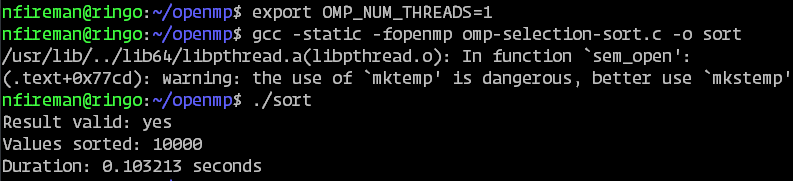
\includegraphics[width=\textwidth]{images/selection-sort-output.png}
\end{exercise}

\begin{exercise}
Re-execute the sorting program with 2, 3, and 4 threads. Which amount of threads yields the fastest execution?
\end{exercise}

\subsection*{Additional resources}

\begin{itemize}
    \item The section \texttt{omp declare reduction} from the "Intel C++ Compiler 16.0 User and Reference Guide":
    
    \url{https://scc.ustc.edu.cn/zlsc/tc4600/intel/2016.0.109/compiler_c/common/core/GUID-7312910C-D175-4544-99C5-29C12D980744.htm}

    \resource{resources/omp-declare-reduction.pdf}
\end{itemize}

\section{OpenMP Tasks}
\label{sec/tasks}

This section will introduce the concept of \emph{tasks} in OpenMP. At a high level, a task is just a block of code that needs to be executed by a single thread, as well as the values of variables that the thread will need to execute the task's code. For example, in a parallelized \texttt{for} loop, each iteration of the loop would be identified as a separate task. Separating each iteration into a separate task is what allows OpenMP to distribute work among many threads in parallel.

In early versions of OpenMP, tasks were only an implementation detail, and not directly accessible to OpenMP programmers. Compiler directives such as \texttt{\#pragma omp parallel} would create tasks under the hood, but a single task could not be explicitly created. In OpenMP version 3.0, the \texttt{\#pragma omp task} directive exposed tasks as part of the OpenMP API.

Through the explicit use of tasks, OpenMP programs are able to share work between threads in more complicated ways than by only using the \texttt{\#pragma omp parallel} directive. For example, the latter does not allow the parallelization of a \texttt{while} loop or a recursive function; tasks allow both.

To demonstrate the use of tasks, the program \texttt{omp-pairwise-sum.c} has been provided, which implements a parallel version of the \emph{pairwise summation} algorithm. This algorithm sums an array of floating-point numbers using a divide-and-conquer approach: the left and right halves of the array are summed recursively, and the sum of the two partial results is the sum of the entire array. In practice, this algorithm has applications when summing arrays of floating-point numbers, since it has been shown to be less vulnerable to round-off error than naively summing the array in order. 

The program uses the \texttt{\#pragma omp task} directive in the \texttt{parallel\_sum} function to parallelize the recursive logic described above. Both recursive calls are placed in \texttt{\#pragma omp task} directives, which allows OpenMP to schedule them in parallel with other recursive calls when possible. Note that since each task is only one statement, the curly braces defining the block can be omitted; this is analagous to when curly braces can be omitted from the body of a \texttt{for} loop.

\begin{verbatim}
// data: the array of input numbers
// count: the number of elements to be added
int parallel_sum(int *data, int count) {
  if (count == 1) return *data;

  int left_sum, right_sum;
  int middle = count / 2;

  #pragma omp task shared(left_sum)
  left_sum = parallel_sum(data, middle);

  #pragma omp task shared(right_sum)
  right_sum = parallel_sum(data + middle, count - middle);

  #pragma omp taskwait
  return left_sum + right_sum;
}\end{verbatim}

By default, variables in a task block are private to that block. Therefore, in order to make sure the values of \texttt{left\_sum} and \texttt{right\_sum} are preserved from each task block to the final line of the function, the \texttt{shared} clauses must be added to each task directive. In general, more than one variable can be shared from a task block using a comma-separated list:

\begin{verbatim}
#pragma omp task shared(var0, var1, var2)
{
  // The three variables `var0`, `var1`, and `var2` are shared
}
\end{verbatim}

While the above program works correctly, its performance is poor as a result of its very high degree of parallelism. In fact, even when \texttt{count} is \texttt{2} (meaning only two numbers from \texttt{data} need to be added), the function will still spawn two OpenMP tasks and attempt to compute the sum "in parallel", which is much slower than simply adding the two numbers in a single thread.

Thus, we can vastly improve the performance of the above function by introducing a \emph{cutoff} array length, where input arrays smaller than the cutoff length will be added serially instead of resorting to task-based recursion. This cutoff value is named \texttt{MIN\_PARALLEL\_COUNT} in the provided program, and serial summation is implemented in the function \texttt{serial\_sum}.

Finally, we turn to how the \texttt{parallel\_sum} function is called from \texttt{main}. As before, since the body of the directives is a single statement, the curly braces can be omitted, even though there are now two nested directives:
\begin{verbatim}
#pragma omp parallel
#pragma omp single
sum = parallel_sum(data, N);
\end{verbatim}

In order to indicate to OpenMP that the \texttt{parallel\_sum} function should be executed with multiple threads, it must be enclosed in a \texttt{\#pragma omp parallel} directive, as we have seen before. But by default, this would execute \texttt{parallel\_sum} once for each thread that is available to the directive. Since \texttt{parallel\_sum} should only be executed once, we also use the \texttt{\#pragma omp single} directive to guarantee that only one thread will actually execute the line of code calling \texttt{parallel\_sum} (usually, the first thread to read the \texttt{single} directive).

\begin{exercise}
\label{exercise/pairwise-sum-1}
Compile and execute \texttt{omp-pairwise-sum.c} with 1, 2, 3, and 4 threads available. Record the execution times in each case. You may need to use the \texttt{-static} argument when compiling with \texttt{gcc}.

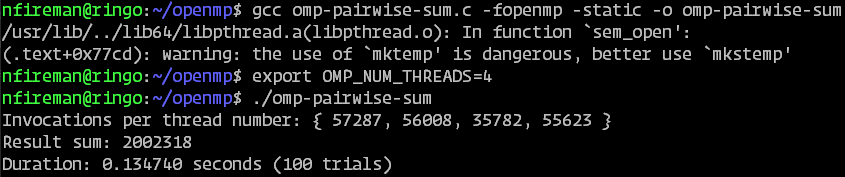
\includegraphics[width=\textwidth]{images/pairwise-sum-output.png}
\end{exercise}

\begin{exercise}
Currently, the cutoff value \texttt{MIN\_PARALLEL\_COUNT} is 1000. With 4 threads available, record the execution durations when the cutoff value is 250 and 4000, and compare the results to Exercise \ref{exercise/pairwise-sum-1}. Try several other values in attempt to further improve the execution duration.
\end{exercise}

\section{Linked list traversal}

This section will demonstrate a linked list traversal algorithm, which will highlight another use case of OpenMP tasks. If the length of a linked list is not known in advance, then traversing it will require a loop with a variable number of iterations. Such a loop cannot be parallelized via OpenMP without the use of tasks. 

The provided program \texttt{omp-linked-list.c} demonstrates the parallelized traversal algorithm. This program uses the following data type for the nodes in our linked list, which contains an \texttt{int} field representing that node's data, as well as a field \texttt{next} pointing to the next node in the list:
\begin{verbatim}
typedef struct node {
  int data;
  struct node* next;
} node;
\end{verbatim}

The function \texttt{construct\_linked\_list} creates a linked list (serially, without the use of OpenMP) of a length given by the passed argument \texttt{length}. This function allocates memory for an appropriate number of \texttt{node} values, links the nodes together via their \texttt{next} fields, and initializes each \texttt{data} field to a random integer value. The last node in the list is made to have a \texttt{next} value of \texttt{NULL} so that it can be identified during traversal. In order to \emph{serially} traverse such a linked list, one could use a loop such as the following:

\begin{verbatim}
node* current_node = construct_linked_list(10);
while (current_node != NULL) {
    // code to process `current_node` belongs here
    
    current_node = current_node->next;
}
\end{verbatim}

When this loop processes the last node in the list, that node will have a \texttt{next} value of \texttt{NULL}, causing the loop to terminate. Given this loop, it should be noted that the actual traversal of the linked list must ultimately occur serially, since the location of a given node can only be computed once that node's predecessor has been traversed first. Thus, this loop should be parallelized only if processing each node is time-consuming relative to the traversal itself. In this case, by packaging the processing of each node into an OpenMP task, the list traversal can be easily parallelized among the threads available to the program.

To parallelize the above loop, we first enclose it in the same \texttt{\#pragma omp parallel} and \texttt{\#pragma omp single} directives that were used in the previous section. As before, the \texttt{parallel} directive makes multiple threads available to work on future tasks that might be created, while the \texttt{single} directive makes sure that the loop is only executed once. Without the \texttt{single} directive, the linked list would be traversed once for each available thread. Inside the \texttt{parallel} directive, the processing of the node is enclosed in a \texttt{task} directive so that OpenMP can distribute that computation to available threads.

\begin{verbatim}
#pragma omp parallel
#pragma omp single
while (current_node != NULL) {
    #pragma omp task
    {
        // code to process `current_node` belongs here
    }
    
    current_node = current_node->next;
}  
\end{verbatim}

Note that in order to simulate a time-consuming computation, this program uses the \texttt{usleep} system call to force each task to wait for a fixed amount of time.

\begin{exercise}
Compile and execute \texttt{omp-linked-list.c} with 1 thread available to the program. You may need to use the \texttt{-static} argument when compiling with \texttt{gcc}:

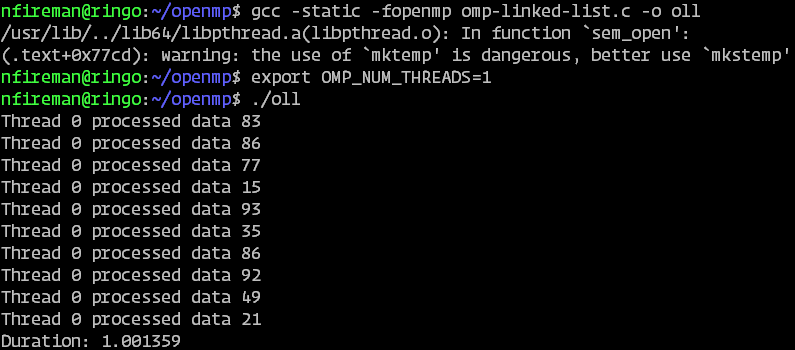
\includegraphics[width=\textwidth]{images/linked-list-output.png}
\end{exercise}

\begin{exercise}
Execute the program with 2 and 3 threads available, and compare the durations to when only 1 thread was used. Predict what the execution time should be if 4 threads were used, then verify your prediction.
\end{exercise}

\begin{exercise}
Comment out the \texttt{usleep} call inside the \texttt{task} directive. After this change is made, processing each node will be very fast relative to the overhead of creating and scheduling tasks introduced by OpenMP, so making more threads available should yield a net decrease in performance. Execute the modified program with 1, 2, and 4 threads available, and record the execution times to confirm that this is the case.  
\end{exercise}

\subsection*{Additional resources}

\begin{itemize}
    \item Section 3.2 of "Using OpenMP—The Next Step" by Ruud van der Pas, Eric Stotzer and Christian Terboven
    
    \resource{resources/using-openmp/3-tasking.pdf}
\end{itemize}

\section{Quicksort}

Quicksort is a popular sorting algorithm that is both relatively simple to implement and performant on common types of data in practice. This section will develop a parallel implementation of quicksort using OpenMP. As in the previous sections, we will see that OpenMP allows us to parallelize a serial implementation of quicksort simply by adding compiler directives, and without modifying the underlying logic of the program.

The main subroutine in quicksort is the \emph{partition} operation, pictured in Figure \ref{fig/quicksort-partition}. One element is chosen as the \emph{partioning element} or the \emph{pivot}, which is the value highlighted in the second row of the figure. To perform the partition, the array is reordered so that all values less than the pivot are left of the pivot, and all values greater than the pivot are to the right of the pivot. After the partition, the pivot value will be located in its correctly sorted position, and sorting the full array is reduced to recursively sorting the left and right subarrays on either side of the pivot.

\begin{figure}
    \centering
    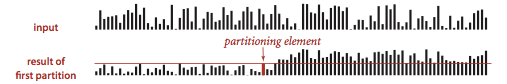
\includegraphics[width=\textwidth]{images/quicksort-partition.png}
    \caption{The effect of one partition.}
    \textbf{Source:} https://algs4.cs.princeton.edu/23quicksort
    \label{fig/quicksort-partition} 
\end{figure}

The provided program \texttt{omp-quicksort.c} implements quicksort using the recursive, divide-and-conquer approach described above. The partition operation is implemented in the \texttt{partition} function, which partitions the subarray of \texttt{data} between the indices \texttt{start} and \texttt{end}:

\begin{verbatim}
int partition(int *data, int start, int end)
\end{verbatim}

In the \texttt{partition} subroutine, the pivot is chosen (arbitrarily) as the middle element of the subarray. It is desirable to choose the pivot as near to the median value of the subarray as possible, and with prior knowledge about the state of the input data, a better choice may sometimes be possible. Note that \texttt{partition} must return the final index of the pivot after performing the partition, since that index also describes the bounds of the two subarrays that need to be recursively sorted. The sorting routine itself is implemented in the \texttt{quicksort} function:

\begin{figure}[H]
\begin{verbatim}
void quicksort(int *data, int start, int end) {
  if (start >= end) return;
  
  int pivot_idx = partition(data, start, end);
    
  #pragma omp task
  quicksort(data, start, pivot_idx - 1);
    
  #pragma omp task
  quicksort(data, pivot_idx + 1, end);
}
\end{verbatim}
\end{figure}

The quicksort routine first partitions the subarray of \texttt{data} between the indices \texttt{start} and \texttt{end}, then recursively sorts the two subarrays on either side of the sorted position of the pivot. The recursive calls are wrapped in task directives, which parallelizes the algorithm as we have seen before.

As we saw in Section \ref{sec/tasks}, using OpenMP tasks carries a certain overhead that can slow a program down when tasks are spawned for very small recursive cases. To remedy this, we can introduce a cutoff length such that calling \texttt{quicksort} on a subarray shorter than the cutoff won't spawn new tasks, and will instead sort the subarray serially. This modification will be performed in Exercise \ref{ex/quicksort-cutoff}.

\begin{exercise}
\label{ex/quicksort-1}
Compile and execute \texttt{omp-quicksort.c} with 1, 2, and 4 threads available. You may need to use the \texttt{-static} argument when compiling with \texttt{gcc}:

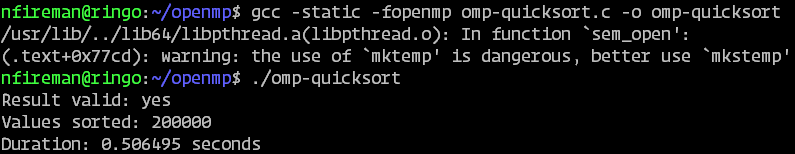
\includegraphics[width=\textwidth]{images/quicksort-output.png}
\end{exercise}

\begin{exercise}
\label{ex/quicksort-cutoff}
Perform the following modifications to \texttt{omp-quicksort.c}:
\begin{itemize}
    \item Create a new function \texttt{serial\_quicksort} that has the same behavior as \texttt{quicksort}, except that it doesn't create new tasks to handle its recursive calls. It should have the same signature as \texttt{quicksort}, namely:\\
    \texttt{void serial\_quicksort(int *data, int start, int end)}
    
    \item Modify \texttt{quicksort} to sort the input subarray by calling \texttt{serial\_quicksort} when the length of the input subarray is below 1000.
    
    \item Compare the performance of the modified program to the performance obtained in Exercise \ref{ex/quicksort-1}.
\end{itemize}
\end{exercise}

\subsection*{Additional resources}

\begin{itemize}
    \item Section 3.3 of "Using OpenMP—The Next Step" by Ruud van der Pas, Eric Stotzer and Christian Terboven
    
    \resource{resources/using-openmp/3-tasking.pdf}
\end{itemize}

\section{Polynomial root-finding}

The problem of \emph{polynomial root-finding} has wide applications in engineering, physics, and other fields. In this problem, we are given an input polynomial $f(x)$:

\begin{equation*}
    f(x) = a_nx^n + a_{n-1}x^{n-1} + ... + a_1x + a_0.
\end{equation*}
We say that $f(x)$ has \emph{degree} $n$, the largest power of $x$ appearing in $f(x)$. Our goal will be to compute the \emph{roots} of $f(x)$, i.e. numbers $r$ so that $f(r) = 0$. $f(x)$ will always have at most $n$ distinct roots (a result known as the Fundmental Theorem of Algebra), but in practice may have anywhere between $0$ and $n$ roots.

Finding the exact values of every root isn't possible in general, but it is for small values of $n$. You may be familiar with the quadratic formula, which tells us the exact roots when $n = 2$; similar \emph{cubic} and \emph{quartic} formulas exist that give exact roots when $n$ is 3 and 4, respectively, but no such general formula exists when $n \geq 5$.

Thus in general, the roots of $f(x)$ must instead be approximated. The simplest such approximation algorithm is the \emph{bisection method}, which has a very similar main idea to a typical binary search. The crux of the bisection method is that one can efficiently identify when an interval $[a, b]$ must contain a root of $f(x)$. Namely, if $f(a)$ and $f(b)$ have opposite signs (either $f(a) > 0$ and $f(b) < 0$, or vice versa), then $f(r)$ must attain the value 0 at some point $r$ between $a$ and $b$. This is illustrated in Figure \ref{fig:bisection-method}.

\begin{figure}[H]
    \centering
    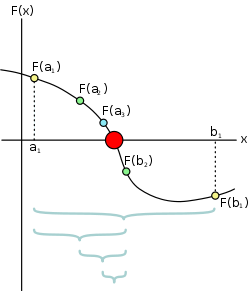
\includegraphics[scale=0.5]{images/bisection-method-illustration.png}
    \caption{Illustration of the bisection method.}
    \textbf{Source:} Wikipedia
    \label{fig:bisection-method}
\end{figure}

Once we know that a root must lie in the interval $[a, b]$, we compute the interval's midpoint $m = \frac{a+b}{2}$ and perform two more tests to determine whether a root lies in the subintervals $[a, m]$ or $[m, b]$. Since these two subintervals cover all of $[a, b]$, the root must lie in one of them. When we identify which subinterval contains the root, we repeat the bisection process again, and so on, until we narrow down the root to a sufficiently small interval.

Since searching one interval for a root in this way is independent of searching any other interval, the bisection method can be naturally parallelized by conducting multiple interval searches concurrently. The provided program \texttt{omp-rootfind.c} contains a parallel implementation of the bisection method, using OpenMP tasks to schedule recursive calls as we have already seen. In terms of the variables used in the program, the interval \texttt{[X\_MIN, X\_MAX]} is searched for roots by splitting this interval into subintervals of width \texttt{X\_STEP}, and using the bisection method to concurrently search for a root in each subinterval.

Note that in general, it is possible for two (or more) roots to go undetected if they lie in the same subinterval of width \texttt{X\_STEP}, since in this case it is possible for the input polynomial to have the same sign on both endpoints of the subinterval. This is a weakness of the bisection method, and the situation of two or more roots very close together can only be resolved by using more a advanced technique.

One complication with the parallel bisection method implemented in this way is that the multiple threads must be able to record each root they find in a shared-memory root list, which must be done in a thread-safe way. In this program, the root list is implemented as a global array \texttt{roots}, and the \texttt{record\_root} function appends a value to this array. To safely append roots without creating a race condition, the \texttt{critical} directive is used to guarantee that only one thread may call the \texttt{record\_root} function at a time:

\begin{verbatim}
#pragma omp critical (root)
record_root((min + mid) / 2);
\end{verbatim}

The \texttt{critical} directive takes an optional \emph{label} argument, which is \texttt{root} in the above code. The label can be used to make multiple blocks of code share the same thread-safe guarantee. Since this program calls \texttt{record\_root} in two different places, the \texttt{root} label is used to prevent one thread recording a root from one call site while another thread is recording a root from the other call site.

\begin{exercise}
\label{ex:rootfind}
Compile and execute \texttt{omp-rootfind.c} with 1, 2, 3, and 4 OpenMP threads. Record the execution time in each case.
\end{exercise}

\begin{exercise}
\label{ex:rootfind-serial}
Modify \texttt{omp-rootfind.c} to run serially by removing both \texttt{\#pragma omp task} directives in the body of the \texttt{find\_roots} function. Compile and execute the modified program with 1, 2, 3, and 4 OpenMP threads. 
\end{exercise}

% \begin{exercise}
% Continuing from Exercise \ref{ex:rootfind-serial}, reparallelize the program using OpenMP directive(s) in the body of the \texttt{main} function. There are several ways of doing this; one way is to rewrite the \texttt{while} loop into a \texttt{for} loop, then add a \texttt{\#pragma omp parallel for} directive. Execute the modified program with 1, 2, 3, and 4 OpenMP threads, and compare the performance to Exercise \ref{ex:rootfind}.
% \end{exercise}

\section{Data pipeline}

This section will demonstrate the \texttt{depend} clause for OpenMP task directives, which allow the programmer to create explicit \emph{dependencies} between tasks. In this context, if task B depends on task A, then task B cannot begin execution until task A has completed its own execution. By using the \texttt{depend} clause in the directives which create tasks A and B, one can guarantee that this ordering will be respected by OpenMP. The following is an example implementation of this two-task scenario using the \texttt{depend} clause:

\begin{verbatim}
int status;

#pragma omp task depend(out:status)
{
  // task A, to be executed first
}

#pragma omp task depend(in:status)
{
  // task B, to be executed after task A completes
}
\end{verbatim}

The variable \texttt{status} is used as a marker to link the dependent tasks. Any variable can be used for this purpose, but in order to create a dependence between tasks, the same variable must be used for each task. Note that the variable itself may or may not be modified by either task; OpenMP only uses its location as the marker, so its usage in the code is independent of its usage as a marker.

The \texttt{depend} clause is used in two different ways in the above code. Modifying a task directive with \texttt{depend(out:status)} means that the modified task can have other tasks which depend on it. Likewise, \texttt{depend(in:status)} means that the modified task depends on tasks with the \texttt{status} marker, and will be performed once a corresponding \texttt{depend(out:status)} task has completed. Thus, by combining both the \texttt{in} and \texttt{out} versions of the clause, a dependence between the two tasks is attained.

The \texttt{depend} clause can be used to parallelize a data \emph{pipeline}, where each section of data is processed in multiple stages that must be completed in a consistent order. By creating a data dependence between each stage of the pipeline, OpenMP can be used to fully parallelize the pipeline, while also making sure to execute the pipeline in the correct order for each section of data.  

The provided program \texttt{omp-pipeline.c} shows a full program which uses the \texttt{depend} clause to implement a two-stage data pipeline. In the first stage, the \texttt{read\_data} function simulates an asynchronous I/O operation by sleeping for a small amount of time, then returns a pointer to an array of integers constituting the read data. The second stage \texttt{process\_data} receives the array of integers from the first stage and computes the sum of its values. A task is created for each stage, and the \texttt{depend} clause is used to guarantee that the stages occur in the proper order:

\begin{verbatim}
int *data_ptrs[i];

for (int i = 0; i < N; i++) {
  #pragma omp task depend(out: data_ptrs[i])
  {
    data_ptrs[i] = read_data(DATA_SIZE);
  }
  
  #pragma omp task depend(in: data_ptrs[i])
  {
    results[i] = process_data(DATA_SIZE, data_ptrs[i]);
  }
}
\end{verbatim}

Here, the elements of the array of pointers \texttt{data\_ptrs} are used as markers for the \texttt{depends} clause. Each iteration of the loop uses a different element as a marker, so each iteration will induce its own two-task dependency chain. 

\begin{exercise}
Add a third stage to the pipeline in \texttt{omp-pipeline.c} that prints the sums stored in \texttt{results}, as follows:
\begin{itemize}
    \item Create a function \texttt{void print\_result(int idx)} that prints \texttt{results[idx]} to the console for a given index \texttt{idx}. 
    
    \item Add a third task directive to the body of the program's main loop which calls \texttt{print\_result(i)}. Use \texttt{results[i]} as a marker to ensure that the second task (which computes \texttt{results[i]}) finishes executing before the newly added third task begins.
\end{itemize}
\end{exercise}

\subsection*{Additional resources}

\begin{itemize}
    \item Section 3.4 of "Using OpenMP—The Next Step" by Ruud van der Pas, Eric Stotzer and Christian Terboven
    
    \resource{resources/using-openmp/3-tasking.pdf}
\end{itemize}

\end{document}
